\documentclass[11pt,a4paper]{article}
\usepackage[utf8]{inputenc}
\usepackage[spanish]{babel}
\usepackage{amsmath}
\usepackage{amsfonts}
\usepackage{amssymb}
\usepackage{graphicx}
\usepackage{subfigure}
\usepackage{alltt}
\usepackage{float}
\usepackage{caption}
\usepackage[left=2cm,right=2cm,top=2cm,bottom=2cm]{geometry}


\begin{document}
\setlength{\unitlength}{1 cm} %Especificar unidad de trabajo
\thispagestyle{empty}
\begin{picture}(18,4)
\put(0,0){
\includegraphics[width=2.3cm,height=3cm]{LOGO.jpg}}
%\put(11.5,0){\includegraphics[width=4cm,height=4cm]{eupinf.jpg}}
\end{picture}
\begin{center}
\textbf{{\LARGE Universidad de Concepci\'on}}\\[0.5cm]
{\Large Facultad de Ciencias F\'isicas y Matem\'aticas}\\[0.5cm]
{\Large Departamento de Estad\'istica}\\[3.5cm]
{\LARGE \textbf{LABORATORIO III}}\\[1cm]
{\LARGE \textbf{DATA MINING}}\\ [4cm]
{\large Nombres: Katerin De la hoz Luna}\\
\hspace{2.2cm}{\large Fernando Pe\~na Villalobos}\\
\hspace{1.7cm}{\large Ariel P\'erez Almonacid}\\[2cm]

{\large Concepci\'on \\
\today}
\end{center}

\newpage

\begin{center}
{\large TRABAJO}
\end{center}

\begin{itemize}
\item[1.] 
\begin{itemize}
\item[a)] A continuación, se muestran los gráficos obtenidos con \verb+plot+ y \verb+qplot+, respectivamente:

\begin{figure}[h]
\subfigure{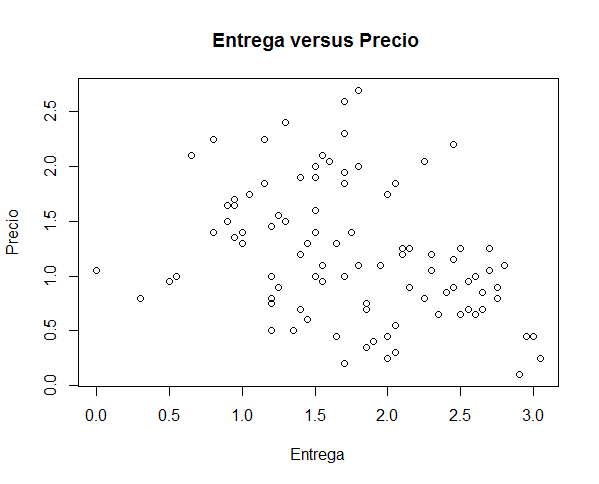
\includegraphics[scale=0.5]{entrega_precio_plot.png}}
\subfigure{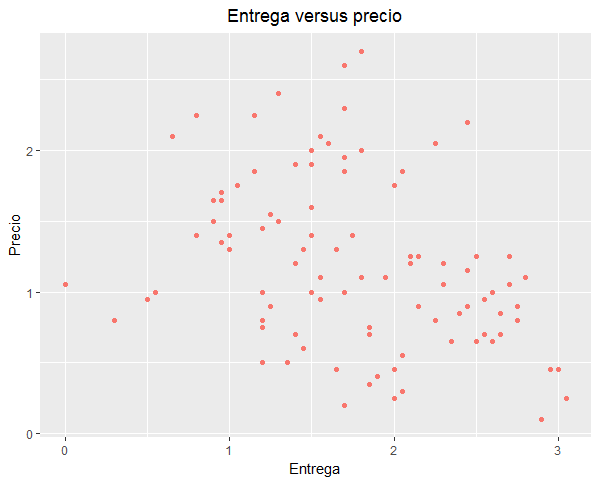
\includegraphics[scale=0.5]{entrega_precio_qplot.png}}
\end{figure}


\item[b)] El gráfico resultantes con \verb+scatterplot3d+ es:
\begin{center}
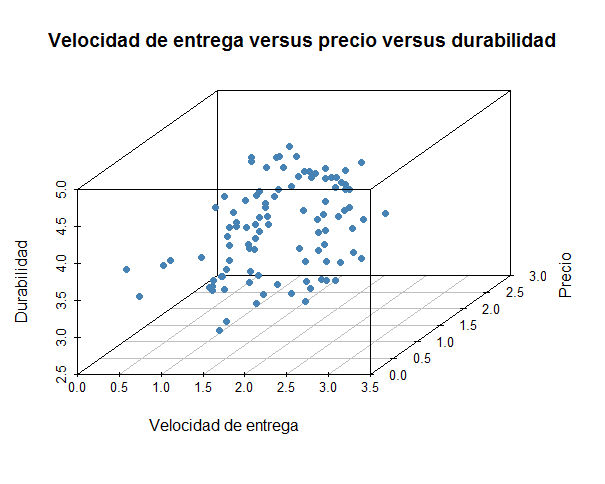
\includegraphics[scale=0.5]{entrega_precio_durabilidad}
\end{center}

\item[c)]Consideremos las siguientes gráficas:

\begin{figure}[H]
\subfigure[]{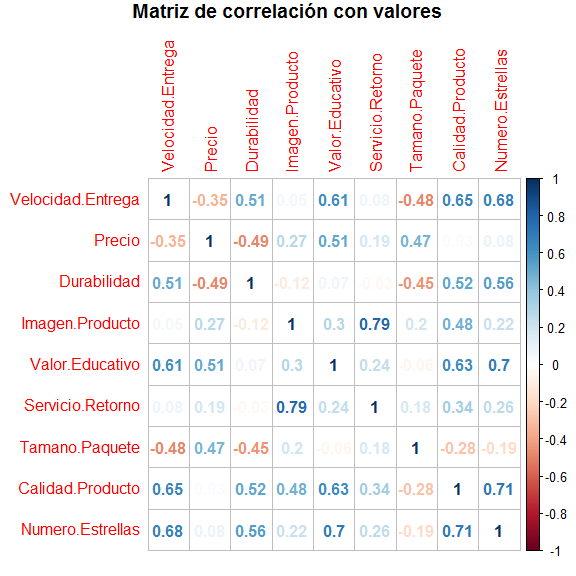
\includegraphics[scale=0.37]{corr_numeros.png}}
\subfigure[]{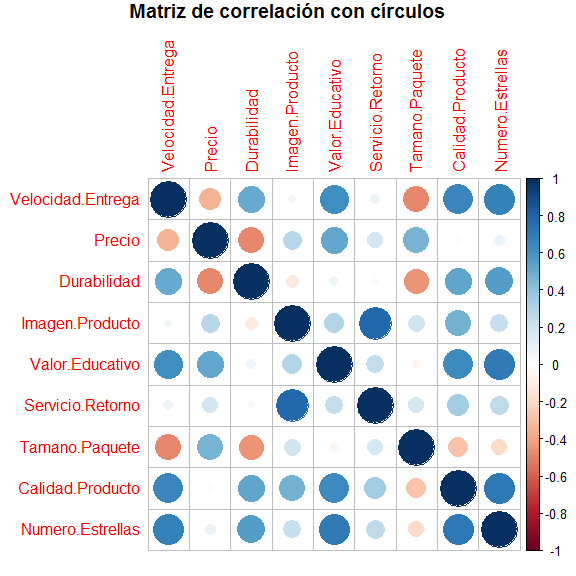
\includegraphics[scale=0.37]{corr_circulos.png}}
\end{figure}

\begin{figure}[H]
\subfigure[]{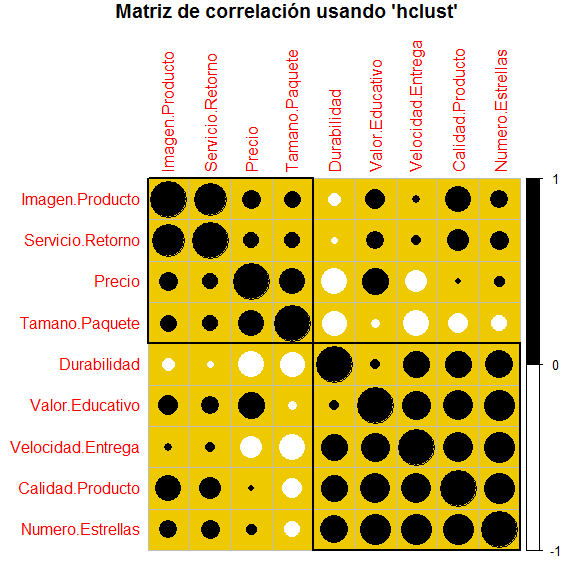
\includegraphics[scale=0.37]{corr_hclust.png}}
\subfigure[]{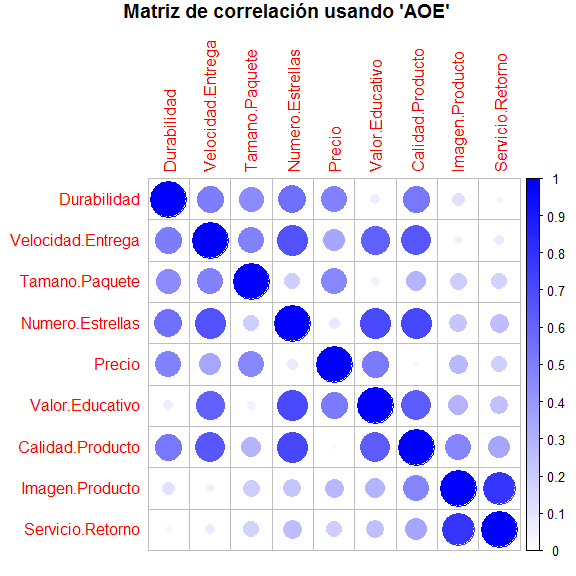
\includegraphics[scale=0.37]{corr_aoe.png}}
\end{figure}

\noindent Las gráficas (c) y (d) muestran la matriz de correlación tal cual fue calculada, la primera lo hace mostrando el valor de cada componente mientras que la segunda muestra círculos de diferentes tamaños dependiendo del valor. Las gráficas (e) y (f) corresponden a un reordenamiento de la matriz, la primera mediante un análisis aglomerativo jerárquico, y la segunda mediante un análisis de valores propios.

\item[d)] Luego de analizar cada variable, se obtuvo que sólo tres características tiene valores atípicos, los cuales se muestran a continuación:

\begin{figure}[H]
\subfigure{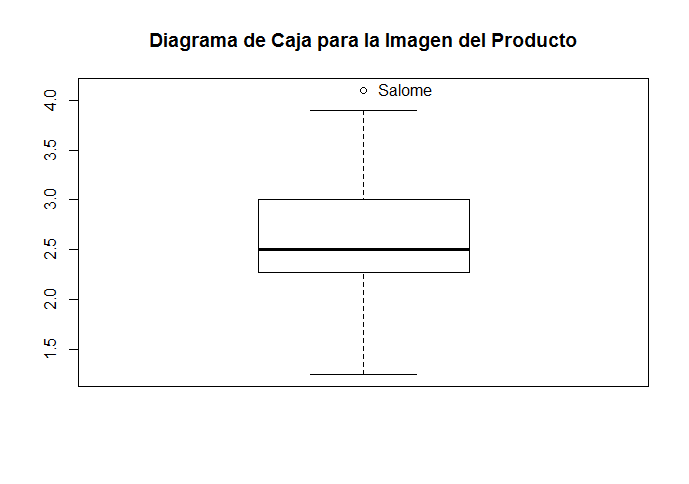
\includegraphics[scale=0.5]{box_imagen_producto.png}}\subfigure{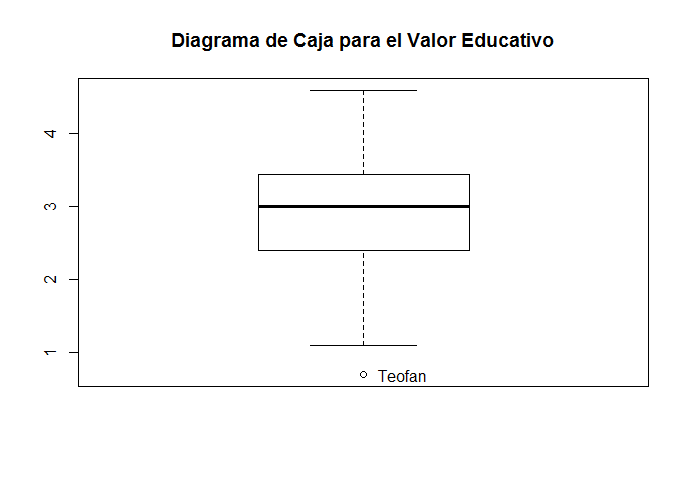
\includegraphics[scale=0.5]{box_valor_educativo.png}}
\end{figure}

\begin{center}
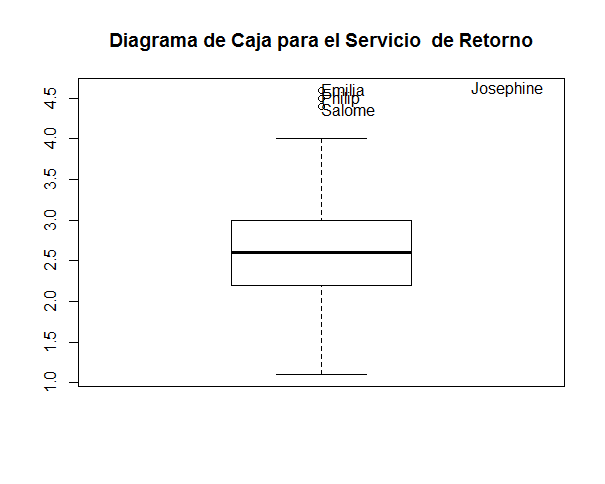
\includegraphics[scale=0.6]{box_servicio_retorno.png}
\end{center}

\end{itemize}
\item[2.] Para comprobar lo pedido ejecutamos lo siguiente:
\begin{verbatim}
> x<-c(1,2,3,4,5)
> y<-1:5
> z<-seq(1,5)
> x==y
[1] TRUE TRUE TRUE TRUE TRUE
> y==z
[1] TRUE TRUE TRUE TRUE TRUE
\end{verbatim} 
Como el resultado de las últimas dos líneas corresponde a verdaderos, por transitividad se tiene que \verb+x=y=z+.
\item[3.] Al definir el vector usando ambos comando se obtienen los siguientes vectores: 
\begin{verbatim}
> y <- c(1,3,5,7)
> y
[1] 1 3 5 7
> z <- seq(1,8,2)
> z
[1] 1 3 5 7
\end{verbatim}
\item[4.] Dado el vector \verb+x+, ejecutando las siguientes instrucciones se obtienen los vectores requeridos.
\begin{verbatim}
x=c(2,-5,4,6,-2,8)
j <- 0
for(i in 1:length(x)){
  if(x[i]>0){
    j<- j+1;
  }
}
y<-integer(j)
j <- 1
for(i in 1:length(x)){
  if(x[i]>0){
    y[j]<-x[i]
    j <- j+1;
  }
}
> y
[1] 2 4 6 8
\end{verbatim}
Entrega el vector de componentes positivas de \verb+x+.
\begin{verbatim}
x=c(2,-5,4,6,-2,8)
j <- 0
for(i in 1:length(x)){
  if(x[i]< 0){
    j<- j+1;
  }
}
z<-integer(j)
j <- 1
for(i in 1:length(x)){
  if(x[i]<0){
    z[j]<-x[i]
    j <- j+1;
  }
}
> z
[1] -5 -2
\end{verbatim}
Entrega el vector de componentes negativas de \verb+x+.
\begin{verbatim}
v<- integer(length(x)-1)
for(i in 1:length(x)-1){
v[i]<-x[i+1]
}
> v
[1] -5  4  6 -2  8
\end{verbatim}
Entrega el vector \verb+x+ sin la primera componente.
\begin{verbatim}
if(length(x)%%2==0){
  w<-integer(length(x)/2)
} else {
  w <- integer((length(x)/2)+1)
}
for(i in 1:length(w)){
  w[i]<-x[2*i-1]
}
> w
[1]  2  4 -2
\end{verbatim}
Entrega las componentes impares del vector \verb+x+. \\
También existen comandos establecidas en R para obtener estos vectores.
\begin{verbatim}
> y <- x[x>0]
> y
[1] 2 4 6 8
> z <- x[x<0]
> z
[1] -5 -2
> v <- x[-1]
> v
[1] -5  4  6 -2  8
> w <- x[-c(2,4,6)]
> w
[1]  2  4 -2
\end{verbatim}
\item[5.] Al especificar sólo el número de filas, se crearán las columnas necesarias para completar la matriz en función del largo del vector dado, como se muestra en el ejemplo:
\begin{verbatim} 
> matrix(1:6,nrow=2)
     [,1] [,2] [,3]
[1,]    1    3    5
[2,]    2    4    6
\end{verbatim}
Si resulta que el número de filas no es un divisor del largo del vector dado, R entrega un mensaje alertando la incongruencia de dimensiones. Sin embargo, la matriz igual se crea, considerando las columnas necesarias de modo que quede bien definida. Ésta se va llenando hasta donde sea posible con los datos, y cuando se acaban, comienza de nuevo, como se muestra a continuación:
\begin{alltt}
> matrix(1:6,nrow=4)
     [,1] [,2]
[1,]    1    5
[2,]    2    6
[3,]    3    \textcircled{1}
[4,]    4    \textcircled{2}
Warning message:
In matrix(1:6, nrow = 4) :
  data length [6] is not a sub-multiple or multiple of the number of rows [4]
\end{alltt}
Lo mismo sucede cuando se define el número de filas y el número de columnas y los datos no se corresponden con la dimensión de la matriz creada. En el caso del ejemplo, para crear la matriz de dimensión $4 x 4$, es necesario utilizar tres veces el vector dado.

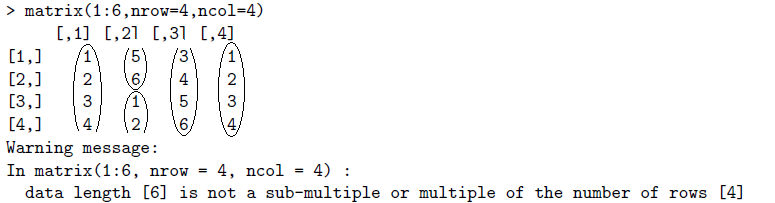
\includegraphics[scale=0.78]{matriz1}
\item[6.] Se tienen los siguientes vectores correspondientes a nombre, edad y sexo.
\begin{verbatim}
> nombre <- c("Ana","Luis","Pedro","Juan","Eva","Jorge")
> nombre
[1] "Ana"   "Luis"  "Pedro" "Juan"  "Eva"   "Jorge"
> edad <- c(23,24,22,24,21,22)
> edad
[1] 23 24 22 24 21 22
> sex <- c("M","H","H","H","M","H")
> sex
[1] "M" "H" "H" "H" "M" "H"
\end{verbatim}
Se convierte el vector sexo en una factor, cuyos niveles son H y M.
\begin{verbatim}
> sexo <- as.factor(sex)
> sexo
[1] M H H H M H
Levels: H M
\end{verbatim}
Finalmente, considerando los vectores anteriores, con la siguiente línea se obtiene lo deseado:
\begin{verbatim}
> amigos <- data.frame(nombre,edad,sexo)
> amigos
  nombre edad sexo
1    Ana   23    M
2   Luis   24    H
3  Pedro   22    H
4   Juan   24    H
5    Eva   21    M
6  Jorge   22    H
\end{verbatim}
\item[7.] Consideremos el siguiente código:
\begin{verbatim}
par(mfrow=c(1,2))
x <- seq(0,2*pi,length=100)
plot(cos(x))
plot(x,cos(x),col="red")
\end{verbatim}
Los gráficos obtenidos para cada comando son, respectivamente:

\begin{center}
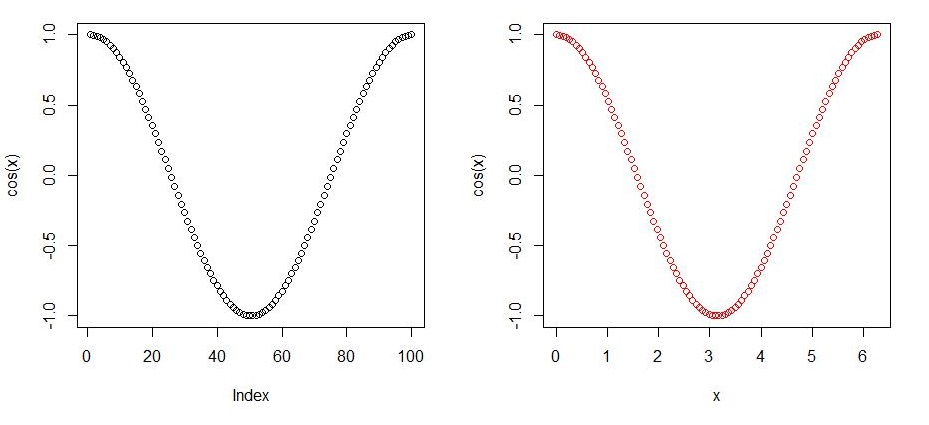
\includegraphics[scale=0.55]{cosenos}
\end{center}

El primer \verb+plot+ grafica index versus $\cos(x)$, donde index es el vector que va desde 1 a 100, el color del gráfico y el estilo son los que vienen por defecto. El segundo \verb+plot+ grafica los valores de $x$ versus $\cos(x)$, donde el estilo es por defecto, y el color es rojo.
\item[8.] Con el siguiente código se obtienen los gráficos necesarios.
\begin{verbatim}
windows(width = 6, height = 7)
par(mfrow=c(2,2))
#(Gráfico 1)
x1 <- seq(0,2*pi, length = 100)
plot(x1, cos(x1), type = "l", col = "red", lwd = 2, xlab = "[0,2pi]", 
     ylab = "y1", cex.axis = 0.9, cex.lab = 0.9)
lines(x1, sin(x1), lty = 2, col = "green", lwd = 2)
title(main = "Seno y Coseno")
legend(0, -0.5, legend = c("Coseno","Seno"), col = c("red","green"), 
       lty = c(1,2), lwd = c(2,2), cex = 0.55, text.width = 0.7)
#(Gráfico 2)
plot(c(1,2,3,4,5), c(1,2,3,4,5), type = "n", xlab = "", ylab = "", 
     main = expression(italic("Título en cursiva")), cex.axis = 0.9)
lines(c(1,2,3,4,5), rep(1,5), col = "green", lwd = 5)
lines(rep(5,5), c(1,2,3,4,5), col = "green", lwd = 4)
lines(c(1,2,3,4,5), rep(5,5), col = "green", lwd = 4)
lines(rep(1,4), c(2,3,4,5), col = "green", lwd = 5)
lines(c(1,2,3,4), rep(2,4), col = "green", lwd = 5)
lines(rep(4,3), c(2,3,4), col = "green", lwd = 4)
lines(c(2,3,4), rep(4,3), col = "green", lwd = 4)
lines(c(2,2), c(3,4), col = "green", lwd = 5)
lines(c(2,3), c(3,3), col ="green", lwd = 4)
mtext("Eje x de color azul", 1, line = 3, col = "blue", cex = 0.7)
mtext("Eje y de color azul", 2, line = 3, col = "blue", cex = 0.7)
text(3, 1.5, expression(bold("Texto en negrita")), cex = 0.7)
#(Gráfico 3)
x2 <- seq(1, 10, length = 100)
plot(x2, log(x2), type = "l", col = "green", xlab = "Coordenada x", 
     ylab = "Coordenada y", main = "Función logaritmo", lwd = 3, cex.axis = 0.9,
     cex.lab = 0.7)
points(6, 1, pch = 17, col = "blue", cex = 1.2)
text(7.4, 1.01, "Punto (6,1)", cex = 0.7)
legend(7, 0.5, legend = "f(x)=log(x)", lty = 1, col = "green", lwd = 3, 
       cex = 0.55, text.width = 0.9)
#(Gráfico 4)
require(plotrix)
x3 <- seq(-4, 4, length = 3)
plot(x3, x3, type = "n", xlab = "", ylab = "", 
     main = "Circunferencias concéntricas", cex.lab = 0.7)
points(0, 0, pch = 16, col = "green")
draw.circle(0, 0, 1, nv = 100, border = "cyan", lty = 1, lwd = 2)
draw.circle(0, 0, 2, border = "yellow", lty = 2, lwd = 2)
draw.circle(0, 0, 3, border = "magenta", lty = 3, lwd = 1)
legend(2, -2.5, legend = c("Radio=1","Radio=2","Radio=3"),
       col = c("green","cyan","magenta"), lty = c(1,2,3), lwd = c(2,2,1),
       cex = 0.55, text.width = 0.8)
mtext("Eje x = [-4,4]", 1, line = 3, cex = 0.7)
mtext("Eje y = [-4,4]", 2, line = 3, cex = 0.7)
\end{verbatim}
\begin{center}
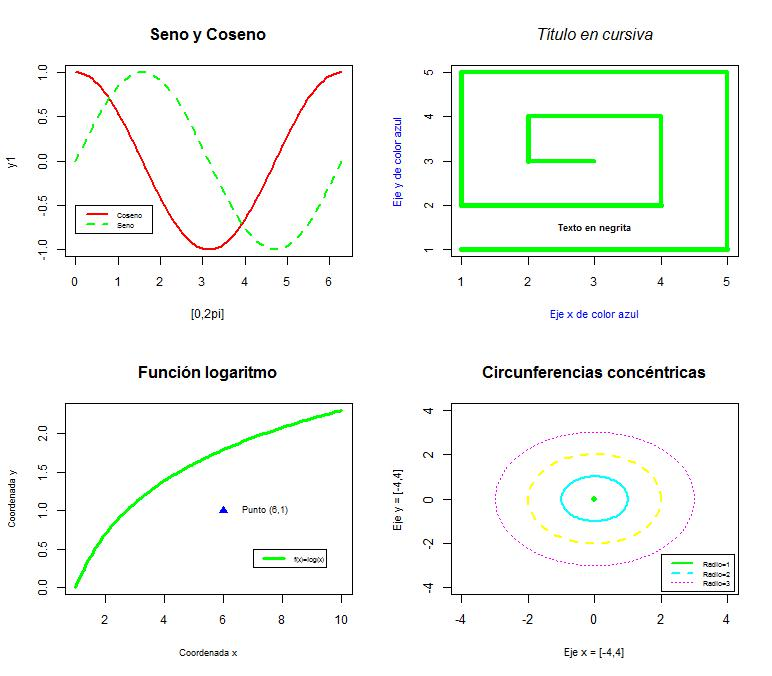
\includegraphics[scale=0.6]{graficos}
\end{center}
\item[9.] 
\begin{verbatim}

#install.packages("ggplot2")
#install.packages("reshape")
library(ggplot2) #carga los paquetes de la librería ggplot2
library(reshape) #carga los paquetes de la librería reshape

head(tips) ##muestra las primeras filas del data frame tips
dim(tips)  ##muestra las dimensiones del data frame  tips 
           ##en un vector de la forma (filas columnas)

##grafica tip (propina) vs total_bill (cuenta total) usando puntos
qplot(tip,total_bill,geom="point", data=tips)

##grafica tip vs total_bill usando puntos 
##y diferenciando si smoker= yes o smoker=no (si es fumador o no)
qplot(tip,total_bill,geom="point", data=tips, colour=smoker) 

##misma gráfica, pero cambiando nombre del eje x e y, además de agregar un título
qplot(tip,total_bill,geom="point", data=tips, colour=smoker, 
      xlab="Tip (in dollars)", ylab="Total Bill (in dollars)",
      main="Scatterplot of Tip by Total Bill,
      Colored by Smoking Status")

##crea un vector con el cuociente entre tip y total_bill en cada componente   
##y lo agrega como una nueva columna, de título rate, a tips 
##(a qué porcentaje de la cuenta equivale la propina)
tips$rate <- tips$tip/tips$total_bill 

##hace un histograma con los "rates" (los agrupa por diferencias de 0.02)
qplot(rate,geom="histogram", data=tips) 

##hace un histograma con los "rates", pero agrupándolos por diferencias de 0.05
qplot(rate,geom="histogram", data=tips, binwidth=.05) 

##lo mismo anterior, pero con bordes negros y color interior celeste
ggplot(tips, aes(x=rate)) + geom_histogram(binwidth=.05,
                                           colour="black", fill="lightblue") 

##Hace un diagrama de cajas sobre los "rates", separando por sexo
qplot(sex, rate, geom="boxplot", data=tips,fill = sex) 

##Mismo diagrama de cajas, agregando título, cambiando nombre al eje x y al eje y, 
##y agregando puntos que muestran cada "rate".
qplot(sex, rate, geom="boxplot", data=tips,
      xlab="Gender", ylab="Tipping Rate",
      main="Boxplots of tipping rate by gender",fill = sex) + geom_jitter() 
\end{verbatim}
\item[10.] El gráfico obtenido es el siguiente:
\begin{center}
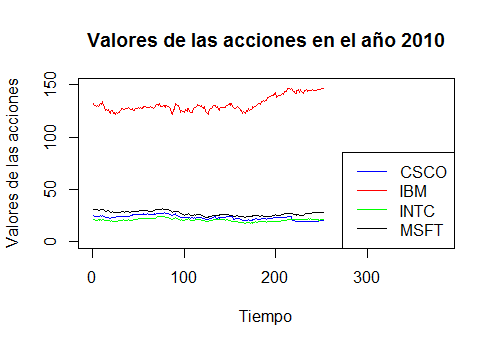
\includegraphics[scale=0.6]{plot}
\end{center}

\newpage
\item[11.] El gráfico obtenido es el siguiente:
\begin{center}
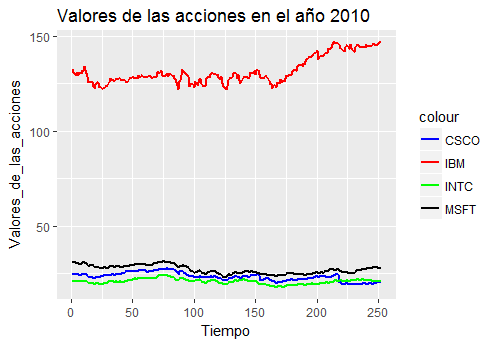
\includegraphics[scale=0.6]{ggplot}
\end{center}
\item[12.]
El primero es un gráfico de puntos donde se relaciona la obesidad con la adiposidad, destacando si se tiene una enfermedad cardíaca o no y separando en dos casos, si hay enfermedades cardíacas en su historial familiar o no. Aquí se observa que un aumento de la obesidad está relacionado con uno de la adiposidad, así como una mayor presencia de enfermedad cardíaca en personas con adiposidad alta.\\
\\
Además, el porcentaje de personas con enfermedad cardíaca es mayor si un familiar tuvo una.
\begin{center}
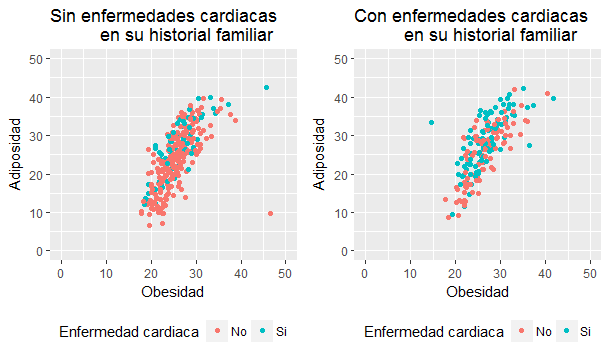
\includegraphics[scale=0.75]{adiposidad}
\end{center}
El código utilizado fue:
\begin{verbatim}
SA<-read.csv("SAheart.csv",header=TRUE,sep=";",dec=".",fill=TRUE)
SA1<-SA[which(SA$famhist=="Absent"),]
SA2<-SA[which(SA$famhist=="Present"),]
p1<-qplot(obesity,adiposity,xlim = c(0,50),ylim = c (0,50),
          xlab="Obesidad", ylab="Adiposidad",main="Sin enfermedades cardiacas
          en su historial familiar",
          geom="point", data=SA1, colour=chd)+theme(legend.position="bottom")+
  labs(colour="Enfermedad cardiaca")
p2<-qplot(obesity,adiposity,xlim = c(0,50),ylim = c (0,50),
          xlab="Obesidad", ylab="Adiposidad",main="Con enfermedades cardiacas
          en su historial familiar",
          geom="point", data=SA2, colour=chd)+theme(legend.position="bottom")+
  labs(colour="Enfermedad cardiaca")
grid.arrange(p1,p2, ncol=2, nrow =1)
\end{verbatim}

Después de leer la tabla, esta se separó en otras dos tablas, una con las personas con presencia de enfermedades cardiacas en su historial familiar y otra sin la presencia.\\
\\
Luego se utilizaron dos qplot, donde se grafica obesidad (eje x) versus adiposidad (eje y), se especifica que los valores en ambos ejes deben ir desde 0 hasta 50, se agregan nombres a estos ejes con los comando xlab e ylab, además de un título con el comando main, se usa geom=point para realizar un gráfico de puntos, data=SA1 (o SA2) hace referencia a que la información se tomará del data frame SA1 (o SA2), mientras que colour=chd se utiliza para diferenciar, con el uso de colores, a las personas que tienen una enfermedad cardíaca de las que no. Posteriormente, se agregó el  comando theme(legend.position="bottom") para que la posición de la leyenda sea en la parte inferior del gráfico y labs para cambiar la etiqueta de la característica dada por el color.\\
\\
Finalmente, se guardó cada plot en una variable (p1 y p2), para finalmente agregar ambos en una misma pantalla con el comando grid.arrange, usando una fila y dos columnas, para que salga uno al lado del otro y sea más fácil la comparación.
\\
\\
En el siguiente se muestran diagramas de cajas, separando en tres grupos según su edad, personas jóvenes (menores de 21 años), adultos (entre 22 y 49 años) y mayores (mayores de 50 años), donde se comparan los niveles de colesterol LDL con la presencia de una enfermedad cardíaca (cuadrado de interior rojo si tienen, amarillo si no), separando si en el historial familiar había o no alguna persona con una (borde celeste si la hay, borde rosado si no). Cabe destacar que en el grupo de los jóvenes no hay una caja de borde azul y relleno rojo, y eso es debido a que en ese grupo no hay personas con enfermedades cardíacas que tengan una en su historial familiar.\\
\\
Se puede observar que, en los jóvenes, las personas con una enfermedad cardíaca la concentración de colesterol LDL es baja. Sin embargo, la muestra de personas jóvenes con enfermedad cardíaca es muy baja como para concluir algo.\\
\\
Además, en promedio, las personas jóvenes tienen una concentración de colesterol LDL menor que los mayores de 22 años.\\
\\
Por otro lado, tanto en personas adultas como mayores, se observa que la presencia de una enfermedad cardíaca en el historial familiar más un colesterol LDL alto viene acompañado de una enfermedad al corazón.\\
\\
Por otra parte, se nota la presencia de muchos datos atípicos, lo que en este caso significa la presencia de gente con una concentración de colesterol LDL mayor a la usual en su grupo de edad, siendo más común en personas adultas (tengan o no una enfermedad coronaria) y menos frecuente en personas jóvenes, donde estos datos no pasarían a ser atípicos si no se hiciera esta separación.
\begin{center}
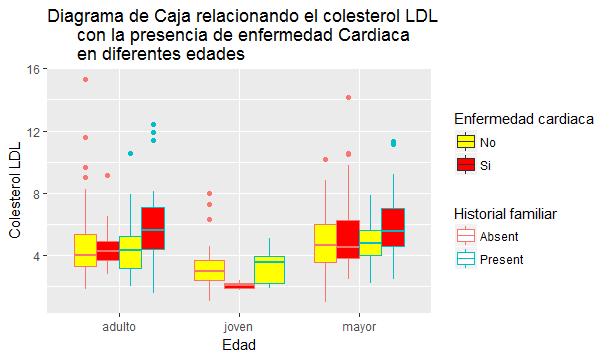
\includegraphics[scale=0.7]{boxplot}
\end{center}
El código utilizado fue:
\begin{verbatim}
SA$tipo <- "joven"
for (i in 1:dim(SA2)[1]){
if (SA$age[i]<22){
SA$tipo[i] <- "joven"
} 
else if (50>SA$age[i]&SA$age[i]>21){
  SA$tipo[i] <- "adulto"
} 
else if (SA$age[i]>49){
  SA$tipo[i] <- "mayor"
  }
qplot(tipo, ldl, geom="boxplot", data=SA,xlab="Edad", ylab="Colesterol LDL",
      main="Diagrama de Caja relacionando el colesterol LDL
      con la presencia de enfermedad Cardiaca
      en diferentes edades",fill = chd,colour=famhist)+
  scale_fill_manual(values=c("yellow", "red"))+
  labs(colour="Historial familiar",fill="Enfermedad cardiaca")
\end{verbatim}

Aquí se comenzó por separar en grupos de edades, agregando una nueva columna al data frame. Luego se realizó un qplot separando por tipo en el eje x (adulto, joven o mayor) y comparando con ldl (colesterol LDL) en el eje y; el comando geom=boxplot (entre comillas) se usó para especificar que el gráfico que se quiere hacer es un diagrama de cajas; con data=SA uno busca los datos del data frame SA; xlab e ylab se utilizan para ponerle nombres al eje x y al eje y respectivamente; main es usado para agregar un título; fill=chd indica que se separarán según el parámetro chd (enfermedad cardíaca) a través del color del relleno de cada caja; con colour=famhist uno separa según el parámetro famhist (si hay enfermedad cardíaca en el historial familiar) con el uso de los colores del borde de las cajas; scale\_fill\_manual es usado para cambiar los colores del relleno, usando dos en este caso debido a que el parámetro chd sólo tiene dos posibles valores (de no hacer esto, los colores usados por defecto serían los mismos que los usados para los bordes); finalmente, con el comando labs, se agregan etiquetas tanto al borde (Historial familiar) como al relleno (Enfermedad cardíaca). Este último comando también pudo haberse usado para agregar el título y las etiquetas a los ejes.\\
\\
 Notar que tanto para  scale\_fill\_manual como para labs se usó un símbolo +, esto es debido a que en el uso de comandos para graficar de la librería ggplot2 se le van agregando características de esta forma (en caso que no estén incluidas en el mismo ggplot o qplot).\\
 \\
Finalmente, se presentan cuatro histogramas, uno considerando la Presión Sanguínea Sistólica, otro el Tipo A, otro el Colesterol LDL y el último la Adiposidad, donde se ve con qué frecuencia una persona presenta una enfermedad cardíaca a medida que aumentas los valores de los atributos previamente mencionados.\\


\begin{center}
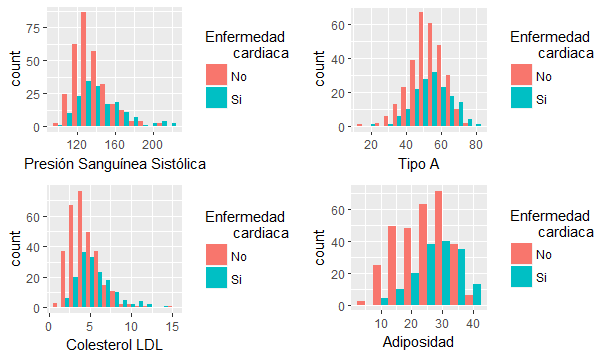
\includegraphics[scale=0.9]{histograma}
\end{center}

El código utilizado fue:
\begin{verbatim}
q1<-ggplot(SA, aes(x=sbp,fill=chd)) + geom_histogram(binwidth=10, position="dodge")+
  labs(x = "Presión Sanguínea Sistólica",fill="Enfermedad
       cardiaca")
q2<-ggplot(SA, aes(x=typea,fill=chd)) + geom_histogram(binwidth=5, position="dodge")+
  labs(x = "Tipo A",fill="Enfermedad
       cardiaca")
q3<-ggplot(SA, aes(x=ldl,fill=chd)) + geom_histogram(binwidth=1, position="dodge")+
  labs(x = "Colesterol LDL",fill="Enfermedad
       cardiaca")
q4<-ggplot(SA, aes(x=adiposity,fill=chd)) + geom_histogram(binwidth=5, position="dodge")+
  labs(x = "Adiposidad",fill="Enfermedad
       cardiaca")
grid.arrange(q1,q2,q3,q4, ncol=2, nrow =2)
\end{verbatim}

Se usaron cuatro ggplot, cada uno guardado en una variable distinta, de la siguiente forma: SA indica que los datos serán sacados del data frame SA, en aes() se ponen los atributos que irán en el eje x (sbp, typea, ldl, adiposity) junto con fill=chd, que indica que se diferenciará con el color del relleno si se cuentan las personas con enfermedad cardíaca o sin ella. Luego, se le suma el comando geom\_histogram(), para indicar que se realizará un histograma, donde en bindwidth se especifica la diferencia de valores según la que se agrupará y position=dodge (entre comillas) es usado para que no se superpongan los conteos. A esto se le vuelve a sumar el comando labs, ya utilizado previamente, para cambiar la etiqueta, en este caso, del eje x y de la leyenda para los colores.\\
\\
Finalmente, se agrega grid.arrange(q1,q2,q3,q4, ncol=2, nrow =2) para ingresar los cuatro histogramas en la misma ventana especificando que serán 2 por columna y dos por filas.


\end{itemize}

\end{document}
